% A LaTeX (non-official) template for ISAE projects reports
% Copyright (C) 2014 Damien Roque
% Version: 0.2
% Author: Damien Roque <damien.roque_AT_isae.fr>

\documentclass[a4paper,12pt]{book}
\usepackage[utf8]{inputenc}
\usepackage[T1]{fontenc}
\usepackage{float}
\usepackage[frenchb]{babel} % If you write in French
%\usepackage[english]{babel} % If you write in English
\usepackage{a4wide}
\usepackage{graphicx}
\graphicspath{{images/}}
\usepackage{subfig}
\usepackage{tikz}
\usetikzlibrary{shapes,arrows}
\usepackage{pgfplots}
\pgfplotsset{compat=newest}
\pgfplotsset{plot coordinates/math parser=false}
\newlength\figureheight
\newlength\figurewidth
\pgfkeys{/pgf/number format/.cd,
set decimal separator={,\!},
1000 sep={\,},
}
\usepackage{ifthen}
\usepackage{ifpdf}
\ifpdf
\usepackage[pdftex]{hyperref}
\else
\usepackage{hyperref}
\fi
\usepackage{color}
\hypersetup{%
colorlinks=true,
linkcolor=black,
citecolor=black,
urlcolor=black}

\renewcommand{\baselinestretch}{1.05}
\usepackage{fancyhdr}
\pagestyle{fancy}
\fancyfoot{}
\fancyhead[LE,RO]{\bfseries\thepage}
\fancyhead[RE]{\bfseries\nouppercase{\leftmark}}
\fancyhead[LO]{\bfseries\nouppercase{\rightmark}}
\setlength{\headheight}{15pt}

\let\headruleORIG\headrule
\renewcommand{\headrule}{\color{black} \headruleORIG}
\renewcommand{\headrulewidth}{1.0pt}
\usepackage{colortbl}
\arrayrulecolor{black}

\fancypagestyle{plain}{
  \fancyhead{}
  \fancyfoot[C]{\thepage}
  \renewcommand{\headrulewidth}{0pt}
}

\makeatletter
\def\@textbottom{\vskip \z@ \@plus 1pt}
\let\@texttop\relax
\makeatother

\makeatletter
\def\cleardoublepage{\clearpage\if@twoside \ifodd\c@page\else%
  \hbox{}%
  \thispagestyle{empty}%
  \newpage%
  \if@twocolumn\hbox{}\newpage\fi\fi\fi}
\makeatother

\usepackage{amsthm}
\usepackage{amssymb,amsmath,bbm}
\usepackage{array}
\usepackage{bm}
\usepackage{multirow}
\usepackage[footnote]{acronym}

\newcommand*{\SET}[1]  {\ensuremath{\mathbf{#1}}}
\newcommand*{\VEC}[1]  {\ensuremath{\boldsymbol{#1}}}
\newcommand*{\FAM}[1]  {\ensuremath{\boldsymbol{#1}}}
\newcommand*{\MAT}[1]  {\ensuremath{\boldsymbol{#1}}}
\newcommand*{\OP}[1]  {\ensuremath{\mathrm{#1}}}
\newcommand*{\NORM}[1]  {\ensuremath{\left\|#1\right\|}}
\newcommand*{\DPR}[2]  {\ensuremath{\left \langle #1,#2 \right \rangle}}
\newcommand*{\calbf}[1]  {\ensuremath{\boldsymbol{\mathcal{#1}}}}
\newcommand*{\shift}[1]  {\ensuremath{\boldsymbol{#1}}}

\newcommand{\eqdef}{\stackrel{\mathrm{def}}{=}}
\newcommand{\argmax}{\operatornamewithlimits{argmax}}
\newcommand{\argmin}{\operatornamewithlimits{argmin}}
\newcommand{\ud}{\, \mathrm{d}}
\newcommand{\vect}{\text{Vect}}
\newcommand{\sinc}{\ensuremath{\mathrm{sinc}}}
\newcommand{\esp}{\ensuremath{\mathbb{E}}}
\newcommand{\hilbert}{\ensuremath{\mathcal{H}}}
\newcommand{\fourier}{\ensuremath{\mathcal{F}}}
\newcommand{\sgn}{\text{sgn}}
\newcommand{\intTT}{\int_{-T}^{T}}
\newcommand{\intT}{\int_{-\frac{T}{2}}^{\frac{T}{2}}}
\newcommand{\intinf}{\int_{-\infty}^{+\infty}}
\newcommand{\Sh}{\ensuremath{\boldsymbol{S}}}
\newcommand{\C}{\SET{C}}
\newcommand{\R}{\SET{R}}
\newcommand{\Z}{\SET{Z}}
\newcommand{\N}{\SET{N}}
\newcommand{\K}{\SET{K}}
\newcommand{\reel}{\mathcal{R}}
\newcommand{\imag}{\mathcal{I}}
\newcommand{\cmnr}{c_{m,n}^\reel}
\newcommand{\cmni}{c_{m,n}^\imag}
\newcommand{\cnr}{c_{n}^\reel}
\newcommand{\cni}{c_{n}^\imag}
\newcommand{\tproto}{g}
\newcommand{\rproto}{\check{g}}
\newcommand{\LR}{\mathcal{L}_2(\SET{R})}
\newcommand{\LZ}{\ell_2(\SET{Z})}
\newcommand{\LZI}[1]{\ell_2(\SET{#1})}
\newcommand{\LZZ}{\ell_2(\SET{Z}^2)}
\newcommand{\diag}{\operatorname{diag}}
\newcommand{\noise}{z}
\newcommand{\Noise}{Z}
\newcommand{\filtnoise}{\zeta}
\newcommand{\tp}{g}
\newcommand{\rp}{\check{g}}
\newcommand{\TP}{G}
\newcommand{\RP}{\check{G}}
\newcommand{\dmin}{d_{\mathrm{min}}}
\newcommand{\Dmin}{D_{\mathrm{min}}}
\newcommand{\Image}{\ensuremath{\text{Im}}}
\newcommand{\Span}{\ensuremath{\text{Span}}}

\newtheoremstyle{break}
  {11pt}{11pt}%
  {\itshape}{}%
  {\bfseries}{}%
  {\newline}{}%
\theoremstyle{break}

%\theoremstyle{definition}
\newtheorem{definition}{Définition}[chapter]

%\theoremstyle{definition}
\newtheorem{theoreme}{Théorème}[chapter]

%\theoremstyle{remark}
\newtheorem{remarque}{Remarque}[chapter]

%\theoremstyle{plain}
\newtheorem{propriete}{Propriété}[chapter]
\newtheorem{exemple}{Exemple}[chapter]

\parskip=5pt
%\sloppy

\begin{document}

%%%%%%%%%%%%%%%%%%
%%% First page %%%
%%%%%%%%%%%%%%%%%%

\begin{titlepage}
\begin{center}


\includegraphics[width=0.6\textwidth]{logo_parisNanterre.png}\\[1cm]
{\large Master MIAGE}\\[0.5cm]
{\large Méthodes Informatiques Appliquées à la Gestion des Entreprises}\\[0.5cm]
{\large Promotion M1 MIAGE Classique}\\[0.5cm]
{\large Année 2017-2018}\\[0.5cm]
%{\large Type de projet}\\[0.5cm]

% Title
\rule{\linewidth}{0.5mm} \\[0.4cm]
{ \huge \bfseries  Développeur au sein du portail de pilotage PPIL\\[0.4cm] }
\rule{\linewidth}{0.5mm} \\[1.5cm]
{\large Client : CNAM (Caisse Nationale de l'Assurance Maladie)}\\[0.5cm]

\includegraphics[width=0.8\textwidth]{logo-soprasteria-2.png}\\[1cm]
% Author and supervisor
\noindent
\begin{minipage}{0.4\textwidth}
  \begin{flushleft} \large
    \emph{Auteur :}\\
    M. Nicolas \textsc{Rouge}\\
  \end{flushleft}
\end{minipage}%
\begin{minipage}{0.4\textwidth}
  \begin{flushright} \large
    \emph{Tuteur de l'entreprise :} \\
    M.~Driss \textsc{IHLALI}\\
    \emph{Tuteur de l'ecole :} \\
    M.~Fabrice \textsc{LEGOND-AUBRY}
  \end{flushright}
\end{minipage}

\vfill

% Bottom of the page
{\large Version 1.0 du\\ \today}

\end{center}
\end{titlepage}

%%%%%%%%%%%%%%%%%%%%%%%%%%%%%
%%% Non-significant pages %%%
%%%%%%%%%%%%%%%%%%%%%%%%%%%%%

\frontmatter

\chapter*{Remerciements}
Je tiens à remercier toute l'équipe PPIL, avec qui j'ai travaillé au quotidien. Toute l'équipe a su m'accueillir et me donner de bons conseils, toujours avec bienveillance. 
Achref a été mon développeur référent. Il a su me donner de bons conseils et suivre ma progression au sein de mon stage. et lors de mes différentes missions de développement.
Je remercie aussi Driss pour son accueil et sa qualité d'écoute.

De nombreuses personnes ont contribué à ma bonne intégration chez Sopra Steria. Grâce notament aux réunions hebdomadaires de stagiaires. Merci à Thomas Richard pour sa présence aux réunions stagiaire, ainsi qu’à tous les stagiaires travaillant pour la Cnam au sein du pôle de Montreuil et à l'Azip.
Je remercie aussi Sara pour le suivi de mon parcours et mon intégration au sein du groupe.
Et enfin merci à toute l'équipe accueil qui a contribué à créer du dynamisme au sein du pôle.

%PPIL : Driss, Nicolas, Arkaia, Huifong, Sonia, Julie, Thomas et Marwan
%
\clearpage
\tableofcontents

\clearpage
\listoffigures

\clearpage
\chapter*{Liste des sigles et acronymes}
\begin{acronym}[CP-OFDMX] % Give the longest acronym here
\acro{SB}{\emph{Solution Builder}}
\acro{BA}{\emph{Business Analyst}}
\acro{PM}{Project Manager}
\acro{CP}{\emph{Chef de Projet}}
\end{acronym}

%%%%%%%%%%%%%%%%%%%%%%%%%%%%%%%%%%%%%%%%%%%%
%%% Content of the report and references %%%
%%%%%%%%%%%%%%%%%%%%%%%%%%%%%%%%%%%%%%%%%%%%

\mainmatter
\pagestyle{fancy}

\cleardoublepage

\chapter*{Introduction}
\addcontentsline{toc}{chapter}{Introduction}
\markboth{Introduction}{Introduction}
\label{chap:introduction}
%\minitoc

Sopra Steria Group m'a accueilli pour mon stage que j'ai effectué dans le cadre de ma formation MASTER 1 MIAGE. Je tenais à effectuer mon stage dans une entreprise novatrice et orienté vers le digital. Ce stage a été pour moi l'occasion d'intégrer la vie active dans le domaine qui me motive. Cela a été ma première expérience de développeur en entreprise.

Lors de ma recherche de stage, je me suis naturellement tourné vers Sopra Steria, entreprise de service numérique qui est un des leader européen de la transformation numérique.
J'ai postulé chez Sopra Steria pour la diversité des projets et des secteurs d'activités ainsi que le grand nombre de métiers. Différentes qualités que l'on retrouve chez les ESN. 

Sopra Steria Group est né de la fusion de deux SSII : Sopra et Steria en Janvier 2015.
L'entreprise intervient sur plusieurs secteurs, chaque secteur est constitué de plusieurs agences qui fonctionnent comme des entreprises indépendantes. 

A la suite d’un entretien j'ai été recruté au sein de l’une des 4 agences du Secteur public : l’agence 151 qui s’occupe du domaine "Santé, Social, Emploi".
Chaque agence est divisée en plusieurs équipes qui gèrent différents projets.

Lors de ce stage, mon objectif était de découvrir le déroulement d'un projet au sein d'une entreprise. Je suis heureux d'avoir pu intégrer une équipe. J'ai pu découvrir tous les aspects de gestion d'un projet, avec les différentes étapes, procédures et les différents rôles que chacun occupe.

J'ai intégré l'équipe PPIL qui développe un outil pour la CNAM. L'outil existe depuis 2010. Il a pour objectif, de permettre en fonction de leurs profils (par exemple Manager ou Chef de projet et bien d'autres) d'effectuer le reporting et le suivi des différents projets. 

Il est primordial de préciser que le client du projet est la CNAM, un des plus gros organisme du secteur public français. L'organisme est en pleine révolution digitale. Sopra Steria Group et ses collaborateurs l’accompagnent sur le chemin de la modernisation.

Travailler pour un client du service public a un intérêt particulier pour moi car les actions menées au quotidien par Sopra Steria ont un impact direct sur la vie de nos concitoyens.

Je suis aussi intervenu sur un projet "stagiaires" interne à Sopra Steria pour le pôle métier de l'agence 151 qui permet la gestion des compétences des différents intervenants du plateau. L'objectif principal de l'outil est de permettre aux chefs de projets ou administrateurs de projets de construire des équipes en fonction des compétences techniques des collaborateurs.

%%% Local Variables: 
%%% mode: latex
%%% TeX-master: "isae-report-template"
%%% End: 

\chapter{Contexte / Environnement}
\label{chap:premierchapitre}

Dans ce chapitre, nous allons présenter l'entreprise dans laquelle j'ai travaillé, Sopra Steria, sa structure, l'agence 151 du secteur public, ainsi que le client auquel nos développement sont destinés : la Cnam.

\section{Sopra Steria}

Sopra Steria est né de la fusion en 2014 de deux des plus anciennes Entreprises de Services du Numérique françaises, Sopra et Steria, fondées respectivement en 1968 et 1969 et marquées toutes deux par un fort esprit entrepreneurial ainsi qu'un grand sens de l’engagement collectif au service de ses clients.

Le Groupe s'affirme comme un des leaders européens de la transformation numérique.

Suite à cette fusion le groupe compte près de 42 000 collaborateurs répartis dans plus de 20 pays et a réalisé un chiffre d’affaire de 3,8 milliards d’euros en 2017.

\begin{figure}[!h]
\centering

\includegraphics[width=0.8\textwidth]{images/chiffres_cles2017.jpg}
\caption{Sopra Steria : leader européen de la transformation numérique}
\end{figure}


Sopra Steria devient alors l'un des leader Européen de la transformation numérique.

\begin{figure}[!h]
\centering
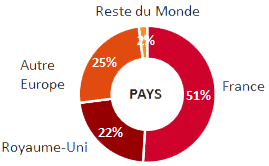
\includegraphics[width=0.5\textwidth]{images/payssoprasteria.png}
\caption{Sopra Steria : Répartition de l'activité en fonction des pays}
\end{figure}

Cette fusion a pris grâce à une forte complémentarité entre les deux entreprises : Sopra Group étant très implanté en France et peu à l'international, et Steria étant une entreprise reconnue à l'international, notamment en Europe.

//L’entreprise intervient dans de nombreux secteurs et domaines d’activité, et a du apprendre à faire face aux problèmes de managements intrinsèquement liés à sa taille et polyvalence.//

\begin{figure}[!h]
\centering
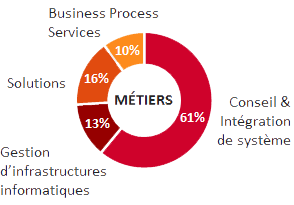
\includegraphics[width=0.5\textwidth]{images/metier_soprasteria.png}
\caption{Sopra Steria : Répartition des activités en fonction des métiers}
\end{figure}

Nous allons expliquer plus en détail les choix organisationnels de l’entreprise en prenant comme exemple notre secteur d’activité.

\section{Organisation du groupe}

//L'entreprise a choisi de diviser les secteurs d’activité et limiter le nombre d’échelons hiérarchiques au sein de chaque secteur, l’entreprise a également donné un grand pouvoir décisionnel et une grande indépendance aux collaborateurs exerçants des fonctions à responsabilités.//

La figure ci-dessous illustre la première division s’effectuant donc par secteur d’activité :

\begin{figure}[!h]
\centering
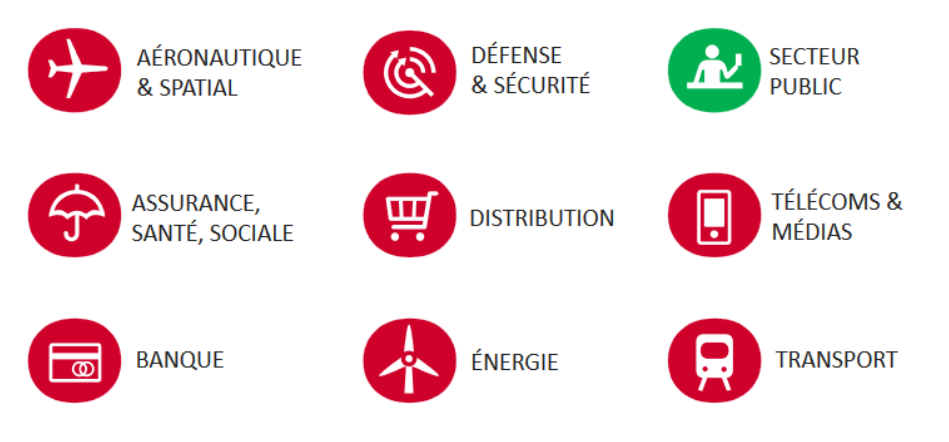
\includegraphics[width=0.8\textwidth]{images/secteurActivite.png}
\caption{Sopra Steria : Secteurs d'activités}
\end{figure}


Une Business Unit (BU) : Secteur public 
Le Secteur Public est le marché majoritaire chez Sopra Steria Group puisqu’il représente 25\% de son chiffre d’affaire.  La Business Unit du Secteur public est réparti sur 4 agences :  

\begin{itemize}
    \item Santé, Social, Emploi : Agence 151 (Sécurité sociale, Pole emploi, CNAMTS…), 
    \item echerche Enseignement : Agence 152 (ministère Éducation nationale, …), 
    \item dministration Centrale : Agence 156 (Mairie de Paris, DGFIP, ONP …), 
    \item onseil : Agence 155 (Clients transverses à toute la BU). Pour ma part, je travaille au sein de l’agence 151, pour le compte de la CNAM.
\end{itemize}


Au sein d'un même secteur d'activité, l'entreprise est divisée en agence qui fonctionnent comme des entreprises autonomes. Elles ont chacun un directeur d'agence, celui-ci dispose d'un grand pouvoir décisionnel au sein de son agence. Son objectif est que l'agence soit performante et fasse des bénéfices.
Une agence prend en charge de nombreux projets, dans notre cas, l'agence 151 gère les missions relevant du domaine de la Santé, du Social et de l’Emploi.
Ci-dessous la division au sein du secteur public.

\begin{figure}[!h]
\centering
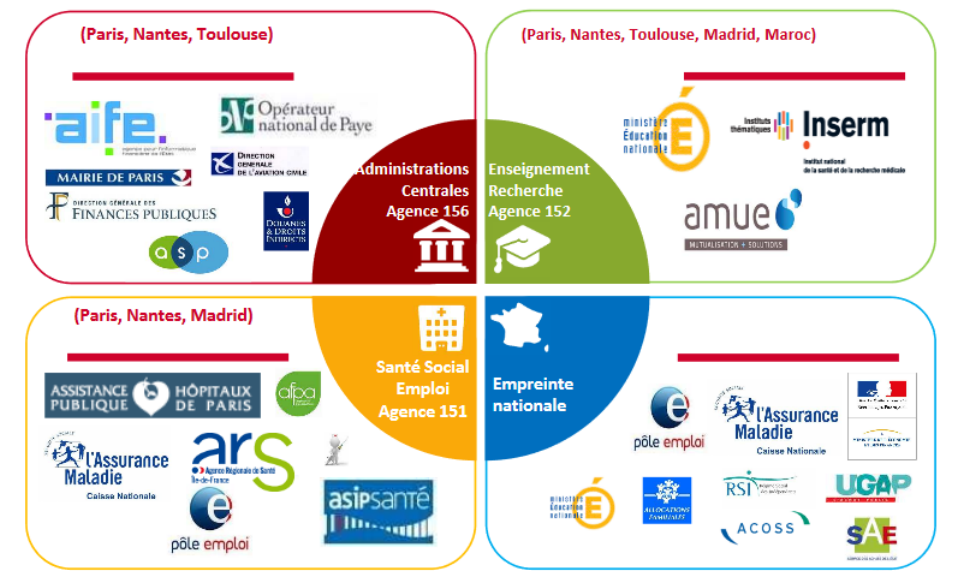
\includegraphics[width=1\textwidth]{images/divisionSecteurPublic.png}
\caption{Sopra Steria : Les agences du Secteur Public}
\end{figure}

\section{L'agence 151}

L'agence 151 est répartie dans plusieurs villes, soit dans les locaux de Sopra Steria, soit directement chez le client.

Les projets sont pris en charge par des équipes, et une équipe peut travailler sur plusieurs projets simultanément, de même plusieurs équipes peuvent travailler sur un même projet. Les équipes sont généralement d’une dizaine de membres, parmi lesquels on retrouve les rôles de :
- Chef de Projet (ou Project Manager),
- Analyste d’affaire (ou Business Analyst),
- Architecte,
- Expert produit (ou Product Expert),
- Solution Builder,
- Commercial.
Mon équipe est installée avec d'autres équipes Sopra Steria dont le client est la Cnam dans les locaux de Sopra Steria dans la tour Cytiscope à Montreuil. 

\section{Le client : la Cnam}

Chez Sopra Steria Group, plus de quatre cent collaborateurs travaillent pour le compte de la CNAM qui génère plus de 40 Millions d’euros de chiffre d’affaire. Ce chiffre est le plus important de toute la BU, ce qui fait de la CNAM un client d’importance maximale pour la société. Pour en dire un peu plus que la Caisse Nationale d’Assurance Maladie (CNAM), elle gère les branches maladie du régime général de la sécurité sociale, et représente :

\begin{itemize}
    \item 57 millions de bénéficiaires affiliés au régime général, 
    \item 4 assurés sur 5, 
    \item 75\% des dépenses de santé. 
\end{itemize}

Sopra Steria Group cherche à aider toutes ces entités en même temps dans leurs tâches quotidiennes. Les équipes de développement web (CNAMTS METIER) et de développement BI (CNAMTS BI) travaillent pour atteindre ces objectifs. Je suis moi même rattaché à la CNAM Métier. Ci-dessous la liste des projets/équipes de la CNAM Métier :

\begin{itemize}
    \item ARPEGE
    \item BIC : Briques I C
    \item CS Nantes
    \item DMP
    \item DPO
    \item DPRA
    \item INDIGO
    \item PPIL : Portail PILotage.
    \item OVERSI
\end{itemize}

\section{Le projet PPIL}
\subsubsection{Un Portail de PILotage}
PPIL permet d'assurer le suivi des projets de la CNAM.
Celui-ci répond à plusieurs besoins :
\begin{itemize}
    \item Centralisation : au sein d’un même espace des données de planification et de pilotage venant de Microsoft Project
    \item Suivi et Contrôle : vues consolidées facilitant le suivi et la vérification des données de pilotage (actualisation des données, cohérence, …)
    \item Évolutivité & Maintenance : socle permettant de mettre en place de nouvelles fonctionnalités et de les déployer pour tous les utilisateurs
    \item Communication : faciliter la diffusion de l’information
\end{itemize}
L'application PPIL a fait l'objet d'une refonte en 2017, désignée sous le nom PPIL V2. 

Les objectifs de cette version sont :
Prioritairement :
\begin{itemize}
    \item Les nouveautés concernant la gestion des projets
    \item Le fonctionnement de l’application PPIL V2 sur socle SharePoint 2013,
    \item L’iso-fonctionnalité par rapport à l’application PPIL V1, à l’exception de quelques fonctionnalités modifiées ou supprimées.
Secondairement :
    \item La simplification du portail,
    \item Des accès aux principales fonctionnalités dès la connexion en fonction des profils utilisateurs,
    \item Un usage simplifié et plus clair des fonctionnalités,
    \item La gestion des droits,
    \item La gestion des référentiels simples,
    \item La gestion des demandes et des lots.
\end{itemize}

Le Portail Pilotage est composé de différents Espaces dont l’accès est conditionné par le profil de l’utilisateur.
Les droits en lecture et/ou écriture selon le profil de l’utilisateur sont visibles dans le document de gouvernance (Gouvernance ci dessous).

Les utilisateurs accèdent à « Mon espace » et selon leurs profils, les informations restituées à l’écran varient. Les sous-espaces définis pour chaque profil suivent la description ci-après, dans l’ordre défini 

\subsubsection{Utilisateurs de PPIL :}
PPIL comprend plusieurs types de profils, on peut citer tout d'abord les profils de type opérationnel, comprenant les : 
\begin{itemize}
    \item Responsable DSI
    \item MOA
    \item Managers (Responsable de Direction ou Responsable de Département) 
    \item Chef de Projet
\end{itemize}
Et on peut citer les profils de type stratégiques, comprenant les :
\begin{itemize}
    \item PMO
    \item Responsable de domaines
\end{itemize}

Il ne faut pas oublier de citer les Visiteurs et Administrateurs.

\subsubsection{Les acteurs et leurs niveaux d'autorisation}
\begin{figure}[!h]
\centering
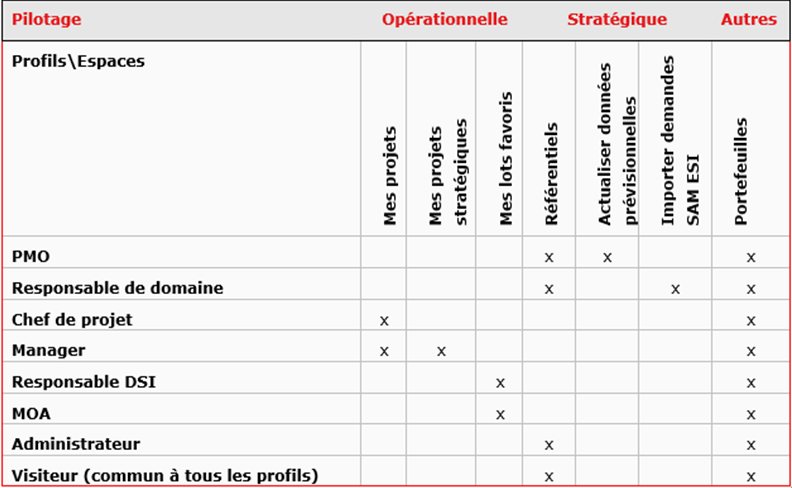
\includegraphics[width=0.8\textwidth]{images/ppil acteurs.png}
\caption{PPIL Les acteurs et leurs autorisations}
\end{figure}

\subsubsection{Lien LOT - Projet - PrtPalier}

(fig. \ref{fig:ppil lien lot projet prtpalier}).

\begin{figure}[!h]
\centering
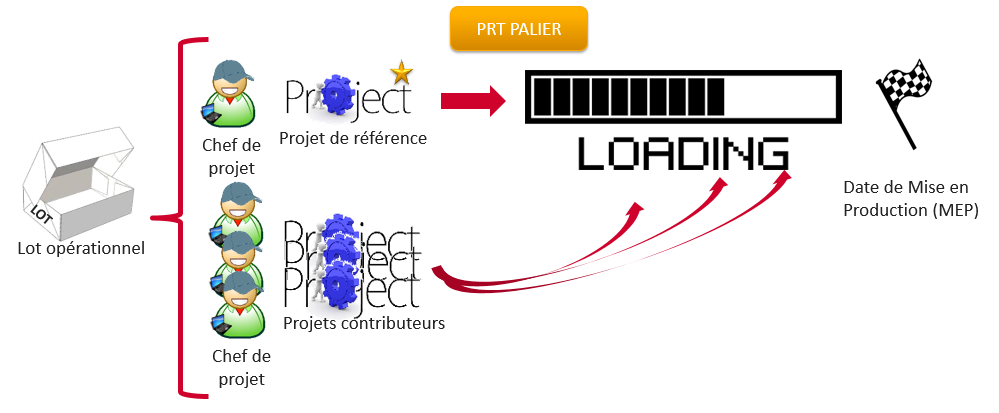
\includegraphics[width=0.9\textwidth]{images/ppil lien lot projet prtpalier.png}
\caption{PPIL lien lot projet PrtPalier}
\end{figure}

\subsubsection{Principe du Reporting - Suivi de projet}

Au sein de la CNAM, tous les acteurs d’un lot renseignent et mettent à jour le planning MSP de leur projet, en renseignant des données du type :

\vspace{1\baselineskip}

\begin{itemize}
    \item Avancement charges, 
    \item Dates des jalons, 
    \item consommé des ressources.
\end{itemize}

\vspace{1\baselineskip}

Les informations MSP sont remontées dans PPIL de plusieurs manières :
\begin{itemize}
    \item Un batch automatique lancé 2 fois par jour
    \item Dans PPIL > Données prévisionnelles
    \item Dans PPIL > Actualiser les données MSP (CP)
\end{itemize}

\vspace{1\baselineskip}

Tous les acteurs doivent renseigner les risques et problèmes rencontrés sur leur projet ainsi que l'état de leur projet (facultatif).

\subsubsection{Principe du Reporting - Exemple du CP}
Le CP du projet référent doit soumettre le reporting du lot toutes les 2 semaines (météo, tendance, situation).

Une fois soumis le reporting du lot est visible par tous les utilisateurs du PPIL.

Le Manager doit saisir la note de conjoncture du lot tous les 2 mois : 
Cette action permet d'expliquer la situation opérationnelle du lot de manière moins technique, cette note de conjoncture est plus destiné aux supérieurs hiérarchiques ( Resp DSI).

\subsubsection{Chef de Projet}

Le Dashboard du CP comprend :

\begin{itemize}
    \item Bulletin de santé
    \item Dérive des jalons
    \item Plan de charges équipe
    \item Accès à la liste de mes projets en cours
    \item Note de conjoncture à mettre à jour
    \item Alertes
    \item Rapports
\end{itemize}

Ci-dessous l'accueil du CP :

\begin{figure}[!h]
\centering
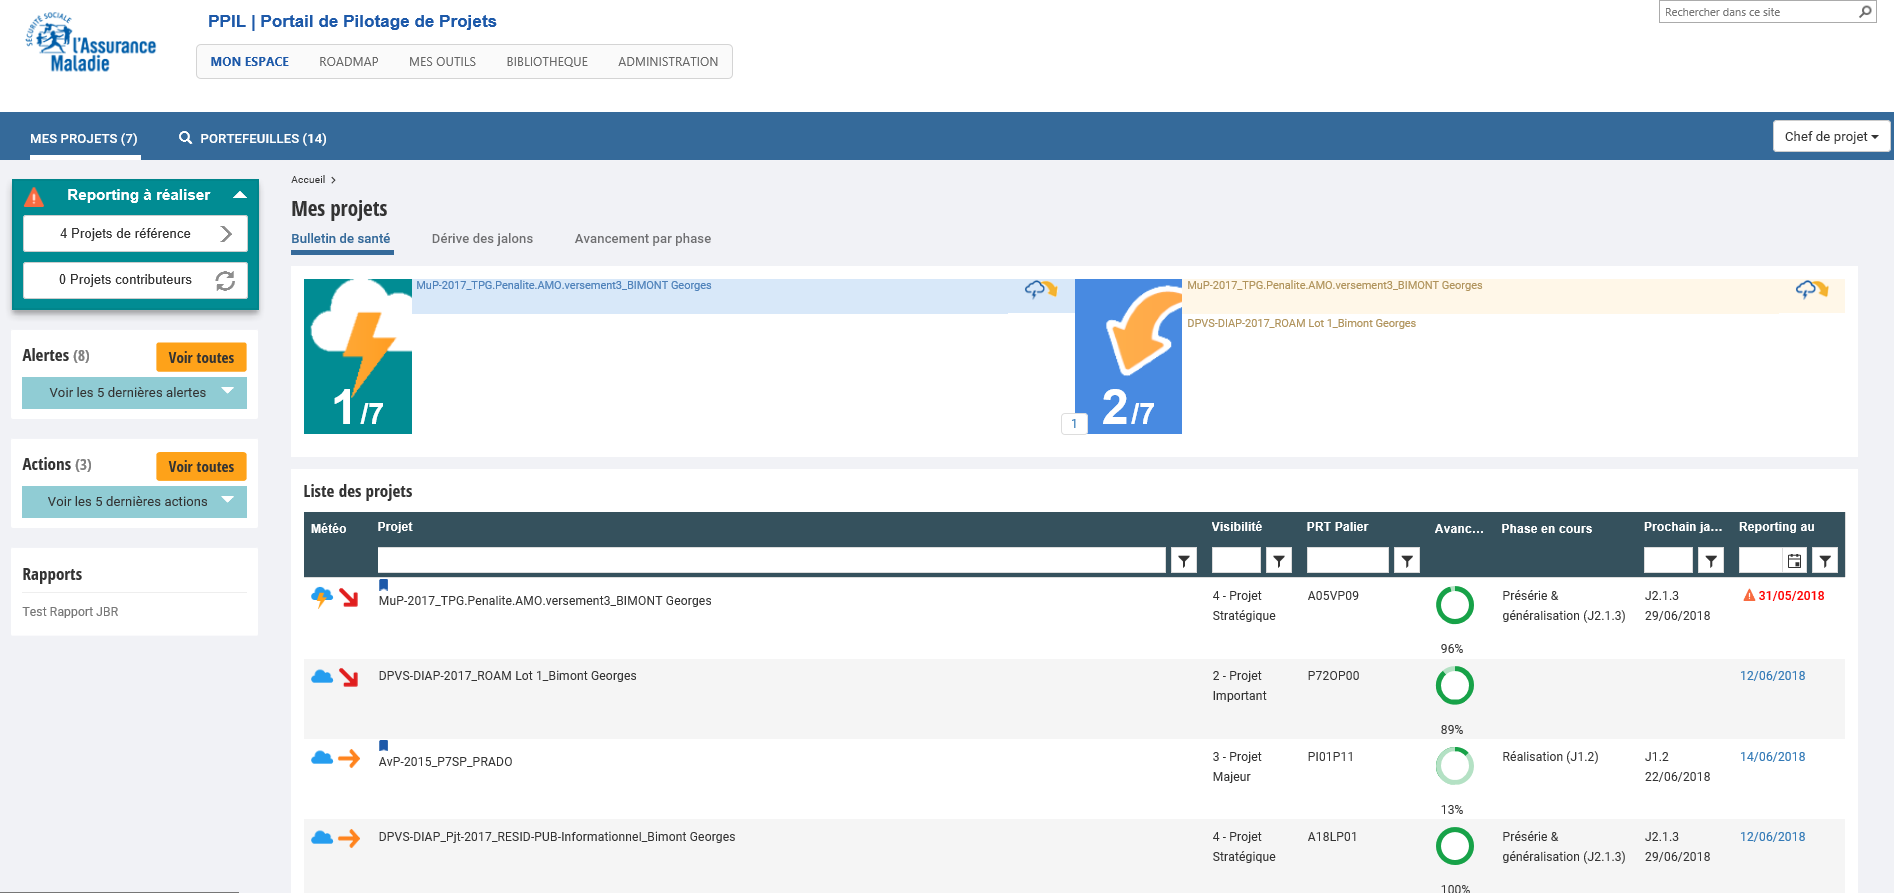
\includegraphics[width=1\textwidth]{images/ppil-CP.PNG}
\caption{PPIL : Accueil CP}
\end{figure}

Ci-dessous, un Chef de projet peut effectuer le reporting d'un projet :

\begin{figure}[!h]
\centering
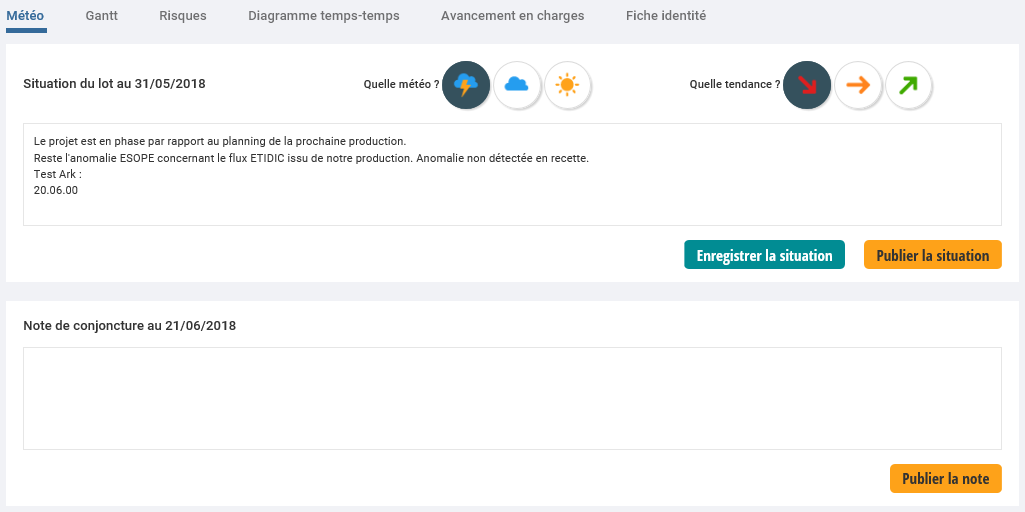
\includegraphics[width=1\textwidth]{images/ppil-meteo.PNG}
\caption{PPIL : Reporting et note de conjoncture}
\end{figure}

On peut aussi avoir accès au portail PPIL via une délégation.

%%% Local Variables: 
%%% mode: latex
%%% TeX-master: "isae-report-template"
%%% End: 
\chapter{Ma mission au sein de PPIL}
\label{sec:unchapitre}

\section{[Objectifs de mission] Intégrer l'équipe PPIL et participer au développement du projet}
Ma mission au cours de ces deux premiers mois de stage a été d'intégrer l'équipe PPIL et de participer au développement du projet. Mes objectifs de mission s'articule autour de trois points :
\subsection{Développement} 
Lors de mes développements, je respecte les règles suivantes :
\begin{itemize}
    \item Acquérir les compétences techniques nécessaires au projet,
    \item Corriger les anomalies affectées par le référent technique sur le périmètre PPIL, 
    \item Garantir aucun retour bloquant en qualification interne et externe,
    \item Garantir la non régression.
\end{itemize}
\subsection{Qualification} 
Les objectifs en terme de qualification sont :
\begin{itemize}
    \item Participer à l'exécution des tests internes avec rigueur dans l'exécution des tests.
    \item Remonter les anomalies détectées. 
    \item Qualifier correctement une anomalie (intitulé, criticité, priorité, type, module, ...) de manière à rendre le plus compréhensible possible l'anomalie, pour le développeur.
\end{itemize}
\subsection{Reporting et Autonomie} 
Lors de mon stage, il est important d'avoir une certaine autonomie, mais aussi de bien s'intégrer dans l'équipe et de savoir quelles informations remonter aux bonnes personnes. Les points que j'ai respecté sont :
\begin{itemize}
    \item Estimer ses charges, suivre son RAE, et le cas échéant expliquer les dérives 
    \item Assurer le reporting auprès de son tuteur et remonter les difficultés rencontrées
    \item Capitaliser ses travaux sur le wiki et le groupe réseau.
\end{itemize}
\section{Fonctionnement de l'équipe}
\subsection{Les différents rôles}
J'ai intégré l'équipe de développement du Portail de PILotage (PPIL) utilisé par les chefs de projet (et autres profils) de la Cnam. L'équipe est composée de 12 collaborateurs. Elle est notamment constituée de :
\begin{itemize}
    \item un CP (chef de projet) 
    \item un RT (référent technique)
    \item un RF (référent fonctionnel)
    \item des BA (business analyst)
    \item des SB (solution builder)
\end{itemize}
Le RT (référent technique) sont les référents fonctionnels, ils gèrent la répartition et l'avancement des tâches de chacun (RAE), il est en contact permanent avec les dév et le CP. Le RF est lui en contact direct avec le client, les BA et le CP.
\subsection{Les processus mis en place}
\subsubsection{processus de livraison}
Les SB (développeurs) développent sur l'environnement de développement.
Les BA disposent de deux environnements de qualification, ils peuvent donc réaliser des tests sur deux versions de PPIL.
A la fin d'un sprint, lorsque les développements évolutions du lot sont terminées, le lot est livré lors d'une "livraison interne" dans l'environnement "qual" de qualification ou les BA peuvent tester la nouvelle version de PPIL.
livraison client = le client teste de son coté avec son équipe;
MEP A la fin d'un lot, mise en production signifie la livraison
sprint de 3 semaines
\subsubsection{processus au sein de l'équipe}
Au sein de l'équipe, nous nous réunissons tous les jours lors des daily-meeting, réunion de courte durée qui permet à chacun des membres de s'exprimer sur son avancement ou ses difficultés. Une fois par semaine toute l'équipe se réuni 1H00 (souvent le vendredi après midi) lors d'un V1. 
Le "V1 PPIL" est constitué de plusieurs points :
\begin{itemize}
    \item Un point sur l'Agence 151 / plateau (le plateau contient une partie de l'agence), des autres projets de l'agence
    \item Un point sur PPIL
    \item Une rétrospective de la semaine, santé du projet, tendance du projet, satisfaction du client
    \item L'évolution du projet, attribution des tâches
\end{itemize}
%%% Local Variables: 
%%% mode: latex
%%% TeX-master: "isae-report-template"
%%% End: 
\chapter{Démarche adoptée et réalisations au sein de PPIL}
\label{chap:premierchapitre}

% --> A ajouter : 
% présentation de PPIL
% indicateurs intéressants. dans montée en compétence : Un projet de gestion de projet
% retour PMO
% mieux rédiger TNR
% mieux rédiger ANO
% vu toute la production d'un projet
%CNAM Métier
%HP ALM

\section{Montée en compétence sur le fonctionnel du projet}

Pendant ma première semaine de stage, j'ai effectué une montée en compétence sur le fonctionnel du projet. Il est important de souligner que j'ai continué à en apprendre toujours d'avantage sur le fonctionnel du projet tout le long de mon stage que ce soit en qualification ou en développement.

Dans cette section, je vais décrire ma démarche pour m'imprégner du projet. Il est évident que cette montée en compétence a été primordiale pour la suite de mon stage.

Pour cela, j'ai utilisé plusieurs méthodes :

Tout d'abord, j'ai étudié les spécifications fonctionnelles et technique du Projet, je me suis aussi procuré le manuel utilisateur de l'application auprès de l'équipe.

Au cours de cette montée en compétence, j'ai posé des questions aux différents analystes fonctionnels du projet, j'ai donc pu bénéficier de les explications des sachant sur le projet : le client, le contexte du projet ainsi que l'histoire de PPIL. 

Quelques informations importantes que j'ai pu recueillir lors de mon arrivée dans l'équipe :
\begin{itemize}
    \item Début de PPIL en 2010, 
    \item Refonte du projet en 2017, 
    \item Exigences du client,
    \item Des sprints qui durent 3 semaines, 
    \item Les besoins et les outils du client (les différents acteurs de la Cnam utilisent MSP),
    \item Comprendre les différentes fonctionnalités de PPIL,
    \item PPIL et les autres projets de la CNAM : on retrouve dans PPIL tous les autres projets de la Cnam,
    \item PPIL est intégré dans SharePoint car les agents de la CNAM manipulent des documents dans leur Sharepoint et le fait d'avoir PPIL dans une même structure leur permet de rassembler plusieurs outils au même endroit.
    \item Fonctionnement du Reporting de PPIL, 
    \item Différents concepts : indicateurs, jalons, diagrammes, lots, projet de référence, projets contributeurs.
\end{itemize}

En plus de ces explications et cette étude des documents, j'ai pu manipuler l'application PPIL, la prendre en main afin de me mettre à la place des utilisateurs finaux et de comprendre comment et pourquoi ils utilisent cet outil qu'est PPIL.

Il a été important de me mettre à la palce des différents profils d'utilisateurs de PPIL :
\begin{itemize}
    \item Chef de projet
    \item Manager
    \item Responsable DSI...
\end{itemize}

A la fin de la semaine, j'ai réalisé une présentation du projet et de ses fonctionnalités aux membres de mon équipe. La présentation a duré 10 minutes, cette présentation a eu pour objectif de présenter tout ce que j'ai appris sur le projet durant la semaine. A la suite de cette présentation, nous avons échangé avec les BA, RT et le chef de projet afin de préciser certains points important dans l'objectif d'en l'objectif que j'en sache un maximum sur le projet.

\subsection{Des indicateurs intéressants en terme de gestion de projet}

Dans cette partie je vais expliquer pourquoi PPIL est très intéressant en terme de gestion de projets. Il permet de voir comment une organisation (la Cnam) gère une multitude de projets.

J'ai découvert dans PPIL le mécanisme de reporting de projets et de lots ainsi que des indicateurs qui permettent de :
\begin{itemize}
    \item Planifier les projets dans le temps (notamment grace aux concept de jalon),
    \item Maîtriser et piloter les risques,
    \item Gérer un grand nombre de projets,
    \item Suivre des enjeux opérationnels de projets ou de lots,
    \item S'adapte en fonction des différents acteurs intervenant dans la gestion de projets.
\end{itemize}

\subsubsection{Visualiser les indicateurs en fonction du profil}

PPIL permet aux différents profils d'utilisateurs de visualiser les informations opérationnelles de leurs projets.

Pour les profils Chef de projet, Manager, Responsable DSI et MOA, on peut visualiser :
\begin{itemize}
    \item Visualiser l’indicateur \textbf{Bulletin de santé}
    Les projets dont la tendance est en dégradation et/ou la météo est orageuse sont mis en évidence par cet indicateur.
    \item Visualiser l’indicateur \textbf{Dérive des jalons}
    \begin{itemize}
        \item Les projets dont le prochain jalon et/ou la date de mise en production est en dérive sont mis en évidence par cet indicateur.
        \item Un jalon est en dérive lorsqu’il existe une différence de plus de 7 jours entre les dates du dernier reporting et de celui fait il y a un mois.
    \end{itemize}
    \item Visualiser l’indicateur \textbf{Avancement par phase} (Chef de projet)
    Les jalons de tous les projets aux états « En cours » du périmètre sont représentés dans cet indicateur.
    \item Visualiser l’indicateur Plan de charge équipe (Manager)
    En cliquant sur le graphique, on accède au rapport du Capacity Planning
    \item Visualiser l’indicateur \textbf{Planning des MEP} (mise en production) : Responsable DSI et MOA
    Les lots dont la date de mise en production est comprise entre le mois passé et les six prochains mois sont placés sur une échelle de temps.
\end{itemize}

\begin{figure}[h]
\centering
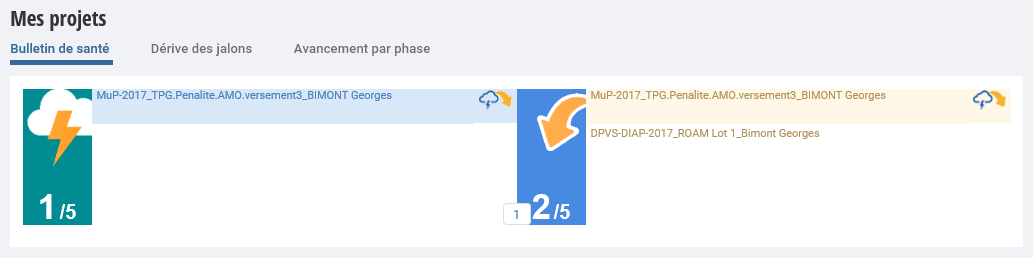
\includegraphics[width=1\textwidth]{images/ppil-bulletion-de-sante.PNG}
\caption{PPIL : Bulletin de santé (Profil Chef de Projet)}
\end{figure}

\subsubsection{Accéder aux reporting / restitution d'un lot / projet}
Pour rappelle, un lot contient plusieurs projets. Dans les indicateurs dans lesquels sont affichés les noms des projets, en cliquant sur le nom d’un projet :
\begin{itemize}
    \item En tant que Manager, Responsable DSI et MOA, on accède à la restitution du reporting
    \item En tant que CP, on accède à la saisie du reporting
\end{itemize}
En accédant au reporting d'un projet, on accède à différents indicateurs intéressants pour un lot/projet : 

\begin{figure}[!h]
\centering
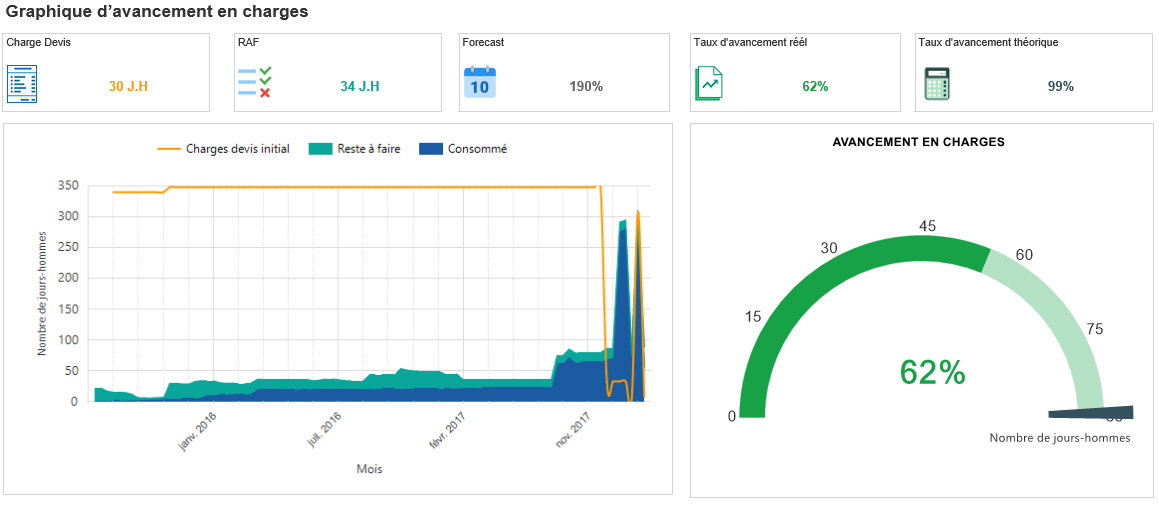
\includegraphics[width=1\textwidth]{images/PPIL-avancement.png}
\caption{PPIL : Graphique d'avancement en charges}
\end{figure}


\begin{figure}[!h]
\centering
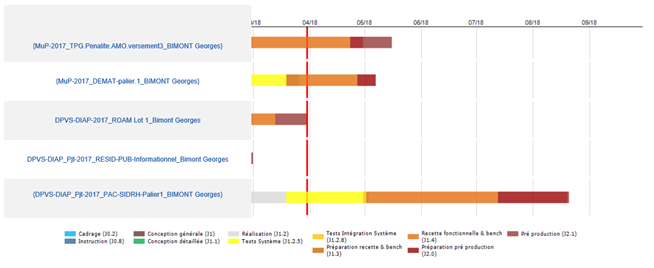
\includegraphics[width=2.5\textwidth]{images/PPIL-Gantt.png}
\caption{PPIL : Gantt des projets contributeurs}
\end{figure}

\begin{figure}[H]
\centering
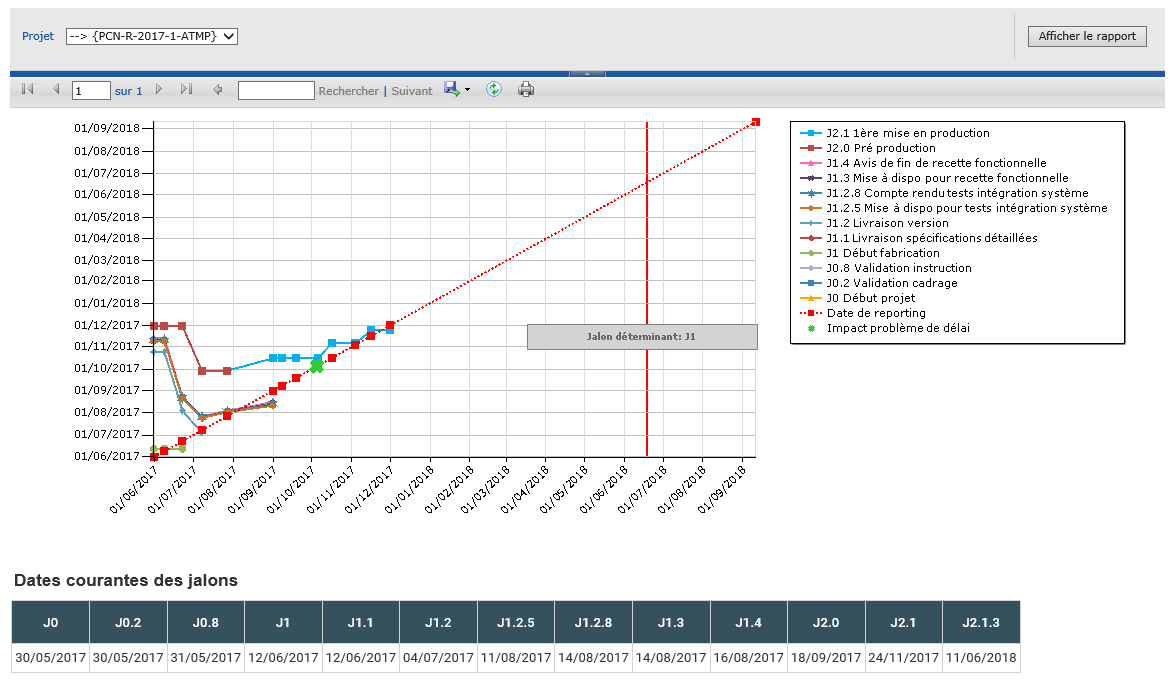
\includegraphics[width=0.8\textwidth]{images/temps temps.png}
\caption{PPIL : Capacity Planning}
\end{figure}

\subsubsection{Exécuter les actions rapides liées à mes projets}
Les actions rapides qui peuvent être effectués en tant que chef de projet sont \textbf{atteindre reporting} et \textbf{Actualiser les données MSP}, et en temps que Manager, on peut visualiser le nombre de notes de conjoncture à mettre à jour.

\subsubsection{Accéder à mes « informations opérationnelles » (CP, Manager, Responsable DSI et MOA)}
Gérer les actions de mes projets
Consulter les actions
Consulter les Facteurs de risque / problèmes
Consulter mes rapports opérationnels
Accéder aux « Rapports »


\section{La qualification}

Une partie de mon stage est destinée à la qualification, j'ai effectué différents tests :
\begin{itemize}
    \item Tests fonctionnels
    \item Tests de Non Régression
    \item Plan de tests
\end{itemize}

\subsection{L'importance des tests}

Durant mon stage, j'ai réalisé des tests afin de vérifier le bon fonctionnement des nouvelles fonctionnalités et corrections du projet ayant pour objectif de détecter d'éventuels anomalies ou régressions. Ces tests m'ont été bénéfique pour comprendre PPIL en profondeur. En effet, pour chaque tests, il faut comprendre et manipuler la base de données du projet, consulter les spécifications techniques ou fonctionnelles (SFG, STD) et poser des questions aux différents membres de l'équipe.

Au cours de ces tests, j'ai rencontré plusieurs difficultés : 

\begin{itemize}
    \item Certaines fonctionnalités à tester ne sont pas évidente à comprendre ou à reproduire.
    \item Les principes de l'outil : par exemple la logique de reporting en fonction des différents indicateurs.
    \item Manipuler une base de donnée complexe. (préparer des jeux de données, changer d'utilisateur, vérifier des informations en base)
\end{itemize}

A chaque fois, ces tests ont été effectués avant une livraison interne ou une livraison client.

Lors des tests il est important de prendre du recul et de tester d'autres fonctionnalités qui pourraient être impactées par la correction qu'on est en train de tester afin de détecter d'éventuels régressions.

Tous ces tests ont été réalisé grâce à l'outil HPALM.
        
Valider un test c'est prendre la responsabilité de dire qu'on peut livrer l'application. L'étape du test est primordiale, sans celle-ci un bon nombre d'erreurs ne seraient pas détectés.

\subsection{Les plans de tests}

J'ai eu l'occasion de rédiger des plans de tests. Cette étape demande une grande rigueur car il est important de couvrir tout le périmètre de la fonctionnalité à tester pour découvrir d'éventuels régressions. Ci-dessous un exemple de plan de test :

\begin{figure}[!h]
\centering
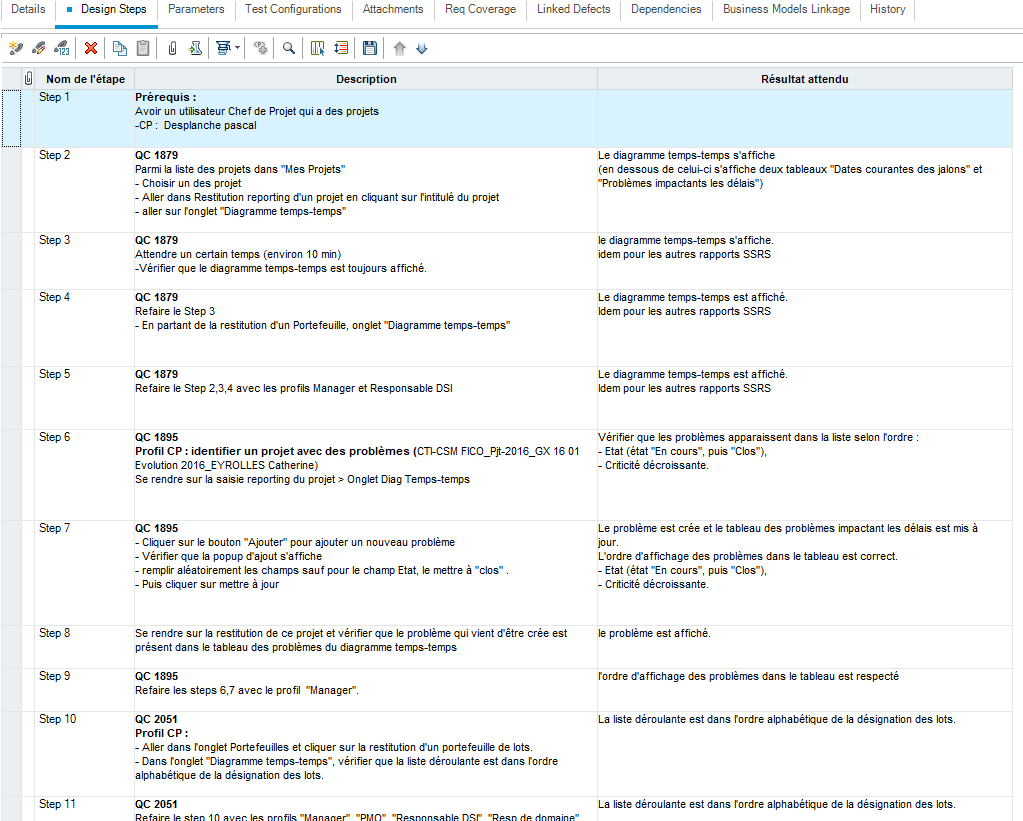
\includegraphics[width=0.8\textwidth]{images/HPLMplantest.png}
\caption{HP LM : Plan de test}
\end{figure}

\subsection{Un exemple de test réalisé : Les tests de Non Régression (TNR)}

[semaine 11/06]
Avant la livraison de la release 20.06.00. Il a fallut effectuer des tests de non régression.

Je vais décrire ici le test "06-TNR-ReportingRestitutionDuLot". Lors de ce test, j'ai détecté trois Defects. Ce qui a permis d'identifier et corriger une anomalie mineure, une anomalie majeure, et une régression majeure. Au cours de ce test de 40 steps, j'ai effectué un grand nombre de requêtes SQL, j'ai dû comprendre la logique de calcul ainsi que la logique d'affichage des indicateurs d'avancement d'un projet en fonction des jalons de celui-ci. Il a fallu que j'analyse la synchronisation des données projet entre Microsoft Project et PPIL.

\subsubsection{Difficultés rencontrées lors de ce test}
%capt ecran

description du step de ce test : 
vérifier que les indicateurs de suivi d'avancement des lots sont corrects :
Dans PPIL, dans la partie restitution de l'avancement d'un projet de référence. Dans cette partie il a fallu comprendre comment sont calculés les indicateurs de restitution pour l'avancement d'un lot. Pour cela j'ai consulté les SFD pour voir les règles de calcul. Je suis allé dans le code chercher les procédures stockées, après cela, j'ai fait mes calculs à l'aide de Excel et de SQL, n'ayant toujours pas le même résultat, j'ai demandé des explications à un BA notamment sur la synchronisation des données de MIcrosoft Project dans PPIL(outil utilisé par les CP de la Cnam pour mettre à jour les jalons de leurs projets). Et j'ai analysé une procédure stockée. Grâce à ces explications et à ces analyses j'ai réussi à ajuster ma requête. 


%Expliquer ce problème
De restitution qui importe les projets contributeurs (qui font parti du même PRT Palier).

Pour la partie Avancement en charge
\begin{figure}[h]
\centering
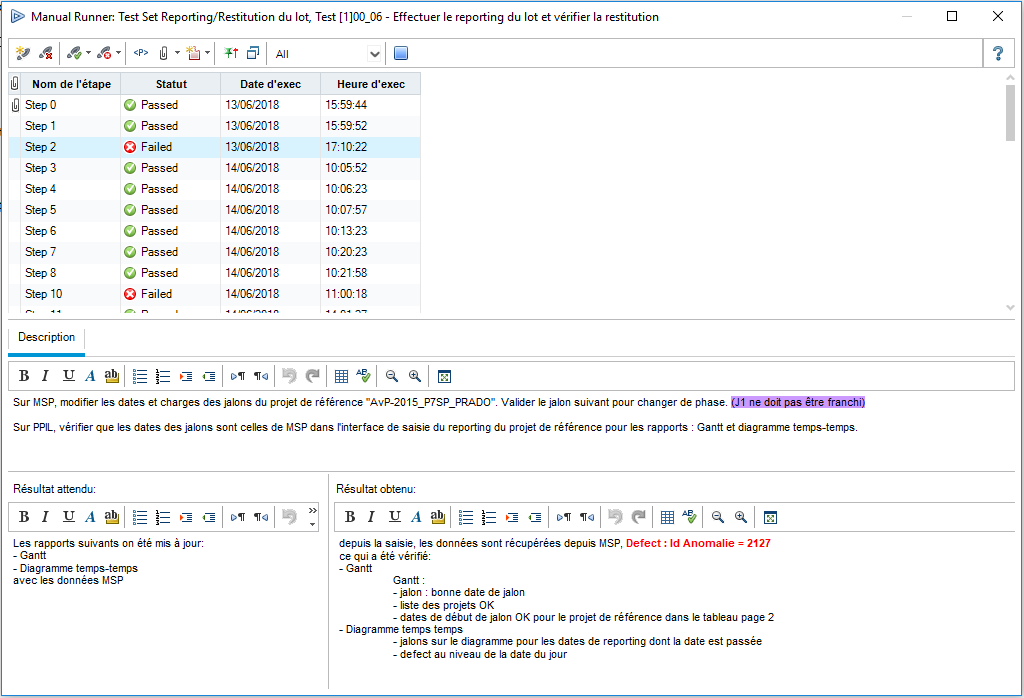
\includegraphics[width=0.8\textwidth]{HPALM-test.PNG}\\[1cm]
\caption{HP ALM : Déroulement d'un test}
\end{figure}

\section{Environnement technique du projet}

Pendant la deuxième semaine, j'ai également mis en place mon environnement de développement avec Achref (mon SB référent). Le projet PPIL se situe dans un contexte technique Microsoft. 

\begin{itemize}
    \item Sharepoint, 
    \item SQLServer, 
    \item .net
    \begin{itemize}
        \item C\#, 
        \item Telerik, 
        \item TypeScrypt, 
        \item Entity Framework, 
        \item SSRS, 
        \item HTML, 
        \item CSS etc).
    \end{itemize}
\end{itemize}

Outils utilisés :
\begin{itemize}
    \item Visual Studio
    \item HPLM
    \item Git
    \item Microsoft SQL Server Management
    \item Microsoft Team Foundation Server
\end{itemize}

\section{Développer au sein de PPIL}

J'ai commencé à développer au mois de Mai. Les développements au sein de PPIL se font en fonction de l'évolution du sprint en cours. Je suis arrivé dans un contexte de correction d'anomalie. C'est naturellement que des (QC) corrections d'anomalies m'ont été attribuées.

Ma première tâche a été de normaliser la charte graphique en même temps que l'interface du projet dans le but d'harmoniser les deux. Cette tâche fait suite à un retour du client (FT). Cela m'a permis de découvrir l'environnement technique. 

Ensuite, j'ai principalement corrigé des anomalies et développé quelques évolutions.

\subsection{Correction d'anomalies}

Lorsque les BA détectent une anomalie, ils l'identifient et la répertorie dans l'outil HPALM. Il est important de préciser que certaines anomalies sont détectées par le client. Elles sont classées par priorité et importance.
Les FT (anomalie retour client) sont souvent prioritaires par rapport aux anomalies détectés par l'équipe.
Un lot correspond à une version de l'application, chaque defect est rattaché à un lot.

\begin{figure}[h]
\centering
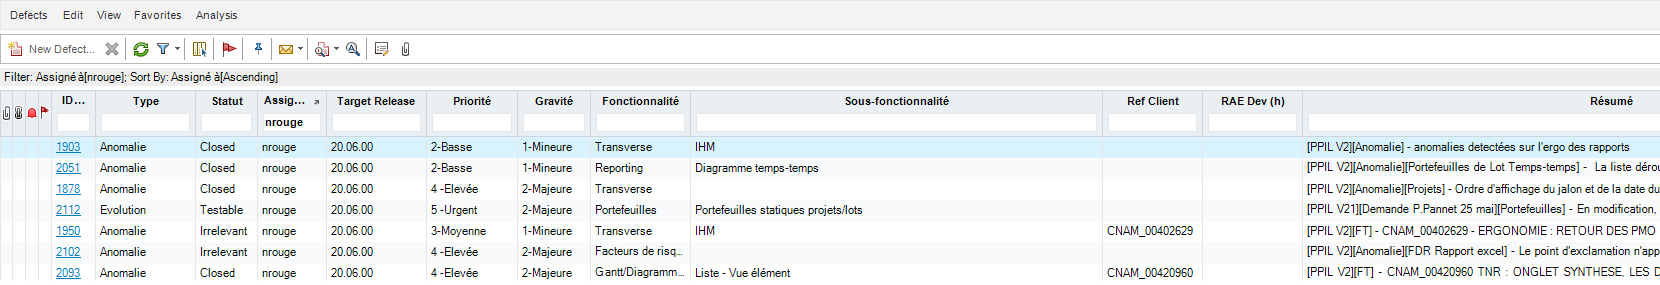
\includegraphics[width=1\textwidth]{images/HPLMliste.png}
\caption{HP LM : Defects corrigés de la release 20.06.00}
\end{figure}

\subsection{Démarche Adoptée}

Avant de commencer le développement, j'ai dû lire les consignes de code, règles à respecter soigneusement car mes développements seront livrés directement.

J'ai été chargé de corriger les anomalies distribuées par les RT.
Le référent technique a attribué différentes QC (Anomalies) aux différents SB. 
Les anomalies que j'ai corrigées étaienent toutes différentes et incluaient différentes technologies à chaque fois.

Quelques exemples d'anomalies que j'ai corrigés : 
\begin{itemize}
    \item Suppression d'un élément qui ne se supprime pas en base
    \item Erreur dans le chargement d'une page
    \item Bouton "annuler" non présent
    \item Ordre ou classement pas correct
    \item Direction de page incorrect lors de la consultation...
\end{itemize}

Pour mener à bien ces différentes corrections, il a été important de prendre du recul avant chaque correction. De bien identifier le périmètre du defect afin d'éviter les régressions.

Tout d'abord, j'ai du comprendre et analyser l'architecture du programme afin d'identifier plus facilement la provenance des defects. 

Chacun des points suivant ont été très important dans ma démarche de correction d'anomalie :
\begin{itemize}
    \item étudier l'architecture de la BDD a été primordiale pour avoir une visibilité sur les relations entre les différentes entités 
    \item me former sur les technos
    \item comprendre l'anomalie aussi bien fonctionnellement que techniquement
    \item analyser l'ampleur et périmètre de l'anomalie
    \begin{itemize}
        \item pour quel type d'utilisateur 
        \item dans quel mode (consultation, restitution, 
        \item dans quel rubrique ( mes projets, ptf, ...
    \end{itemize}
    \item identifier la provenance du problème

\end{itemize}

Comprendre la logique de développement :
\begin{itemize}
    \item comprendre pourquoi le projet a été codé de cette manière
    \begin{itemize}
        \item aller voir les développeurs, 
        \item aller voir le référent technique,
        \item consulter spécifications techniques ou fonctionnelles
    \end{itemize}
    \item identifier les solutions possibles
    \item choisir la meilleure façon de faire à :
    \begin{itemize}
        \item modifier au minimum le code,
        \item trouver la solution la plus optimale,
        \item éviter faire de régression 
    \end{itemize}
 \end{itemize}              
            
\subsubsection{Respect des délais (RAE)}
Pour chacune de mes tâches j'ai dû estimer le temps prévu à la réalisation de celle-ci. Respecter les délais est très important sur plusieurs points :
\begin{itemize}
    \item Pour le projet, cela sert de savoir quand on pourra proposer une version du projet au client.
    \item Pour l'équipe afin de savoir quelle tâche est assignée à quel développeur. 
    \item Pour moi, dans le choix de la démarche de résolution de la tâche.
\end{itemize}

Processus et outil utilisés :
\begin{itemize}
    \item Après avoir développé une évolution les étapes à suivre sont :
    \item "Pusher" ma branche avec git sur le dépot distant,
    \item Créer une "pull request" pour alerter le référent technique,
    \item Commenter la correction ou l'évolution sur HPLM
\end{itemize}

\begin{figure}[!h]
\centering
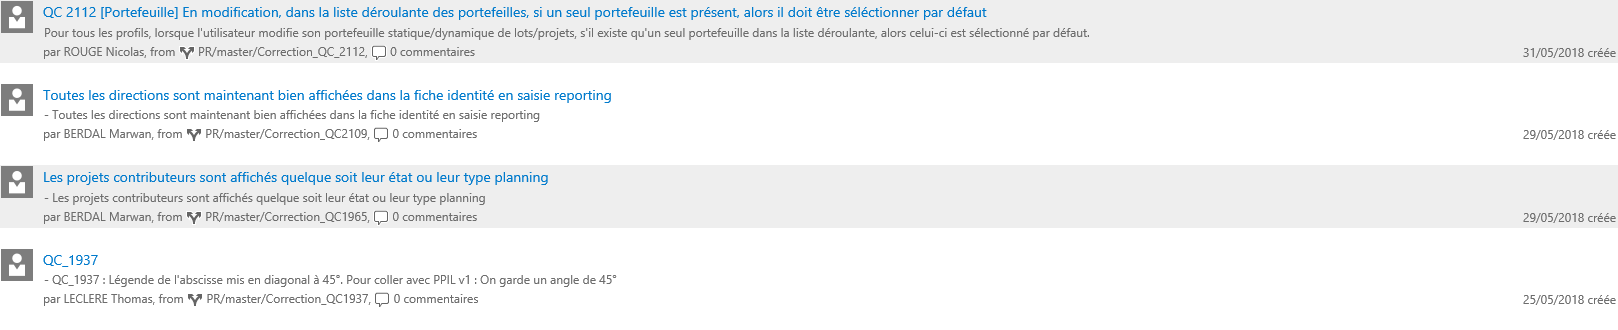
\includegraphics[width=1\textwidth]{images/PullRequest.png}
\caption{Visual Studio Team Foundation : Les Pull Request}
\end{figure}

Ci-dssous le workflow des anomalies dans HP ALM :
\begin{figure}[!h]
\centering
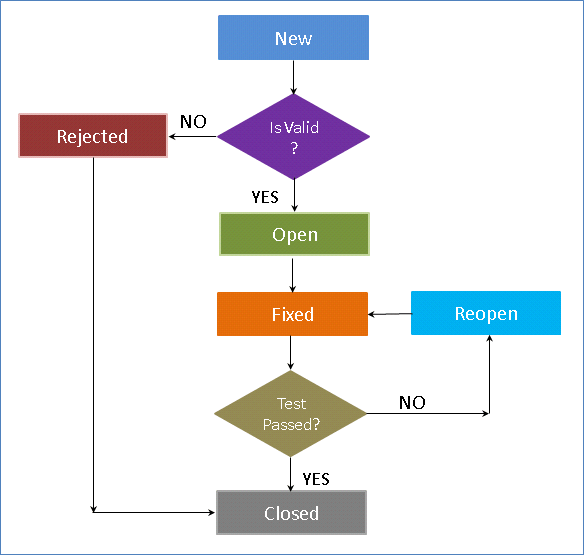
\includegraphics[width=0.6\textwidth]{images/DefectHPALM.png}
\caption{HP ALM Defect Workflow}
\end{figure}

\subsection{Quelques exemples d'anomalies corrigées}

Toutes les anomalies ont été intéressantes à corriger, et elles m'ont fait progresser et travailler sur des technologies diverses. J'ai réussi à acquérir les compétences techniques et nécessaires au projet. L'enjeu de la correction de ces anomalies c'est de n'avoir aucun retour bloquant en qualification interne et externe ainsi que de garantir la non régression.

\subsubsection{Anomalie [Poretefeuille][liste déroulante]}

Visuel de l'anomalie dans HPALM :
\begin{figure}[!h]
\centering
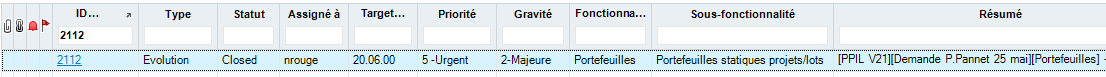
\includegraphics[width=1\textwidth]{images/QC2120.PNG}
\caption{HPALM : Defect 2112}
\end{figure}

On peut voir que l'anomalie est de priorité urgente et de gravité majeure, et qu'elle a été détectée par le client (priorité supplémentaire).

\textbf{Description de la correction à effectuer :} 

[Profil CP ou Manager][portefeuille]
Dans la liste déroulante qui apparaît lorsqu'on veut ajouter des projets ou des lots dans les différents portefeuilles de : 

\begin{itemize}
    \item lots statiques,
    \item lots dynamiques,
    \item projets statiques,
    \item projets dynamiques.
\end{itemize}

Sélectionner par défaut un portefeuille s'il n'y en a qu'un seul. Ne rien sélectionner par défaut sinon. 
[Profil Responsable DSI][portefeuille], Sélectionner par défaut "Mes projet favori" quelque soit le nombre de portefeuille existant.

Avant de commencer la correction du code de cette QC, j'ai mis au courant le référent technique que la description du defect était sujette à interprétation.Le RT a remonté l'information au client, qui a fait un retour en précisant le defect.

Lors de la correction en elle-même, j'ai du identifier ou faire les modification de code. Puis au cours de celle-ci j'ai pu monter en compétence sur du C\#, du Type-script ainsi que Kendo. J'ai du prendre en compte les différentes conditions pour réaliser différentes actions. 

\begin{figure}[!h]
\centering
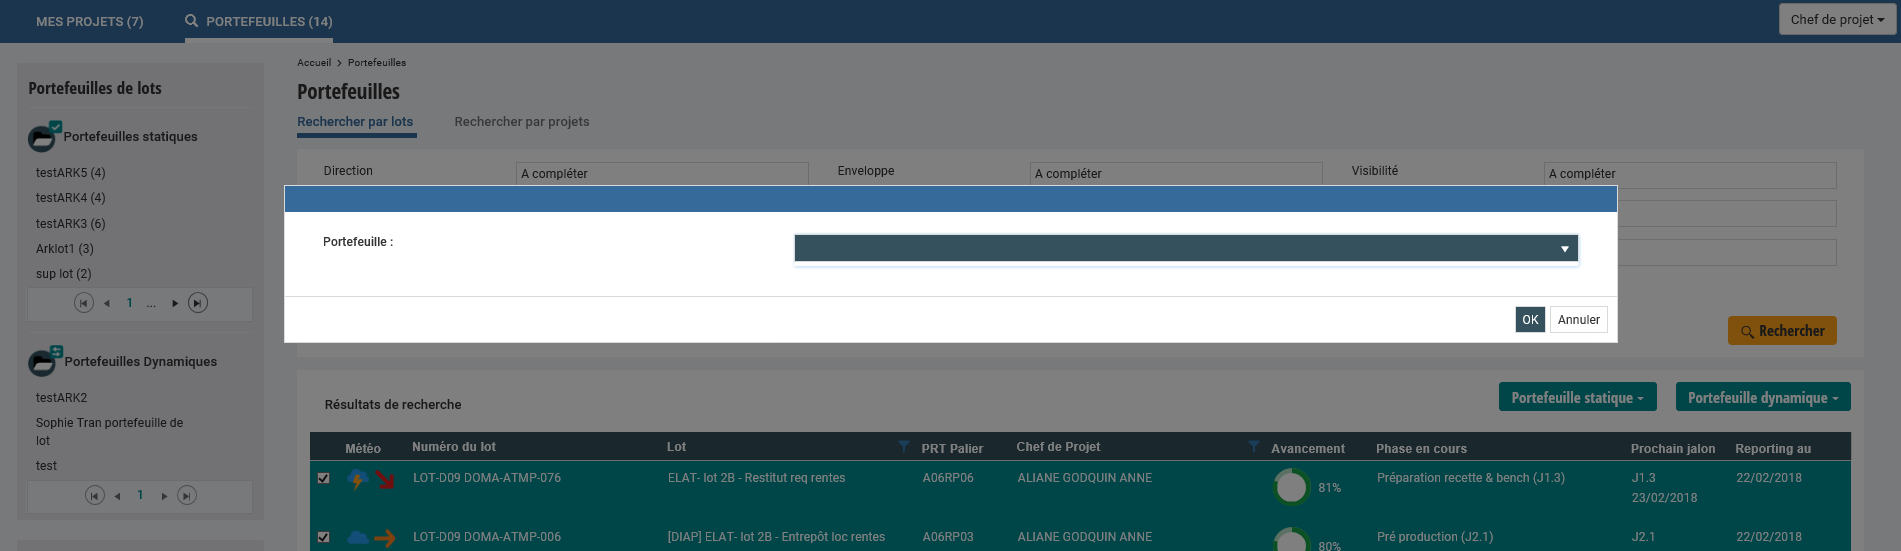
\includegraphics[width=1\textwidth]{images/correction1.PNG}
\caption{HPALM : Defect 2112}
\end{figure}

\subsubsection{Anomalie [Supression des lots non effective dans plusieurs cas]}

\textbf{Description de la correction à effectuer :} 
La suppressions des lots non effective selon certains critères :
\begin{itemize}
    \item Un lot ne se supprime pas quand il est dans un portefeuille (le lot se supprime visuellement mais pas en base, quand on refresh la page il réapparaît)
    \item Un lot ne se supprime pas quand il a des demandes rattaché
    \item Un lot ne se supprime pas quand il n'a pas de projet de référence
\end{itemize}

Cette anomalie m'a pris plusieurs jours de correction, les points importants à souligner sont : 
\begin{itemize}
    \item Il a fallut mettre en place plusieurs jeux de données pour visualiser l'anomalie.
    \item Pendant la correction j'ai détecté une autre anomalie : un lot sans projet de référence ne s'affiche pas dans un portefeuille. (Anomalie que j'ai corrigé par la suite.)
    \item J'ai proposé une solution efficace et correcte.
    \item Je suis allé voir Nicolas (le RT du projet), afin d'avoir son retour sur ma correction.
    \item Il m'a apporté son recul et son expérience en me proposant de refaire une partie de cette correction en modifiant une procédure stockée en SQL plutôt que de modifier une partie du code. Cette solution étant préférable pour la maintenabilité du code et de l'optimisation**.
\end{itemize}

Pour rappel, ce sont les PMO qui ont les droits pour supprimer des lots, un lot est constitué d'un ensemble de projets. Ci-dessous l'interface des PMO.

\begin{figure}[!h]
\centering
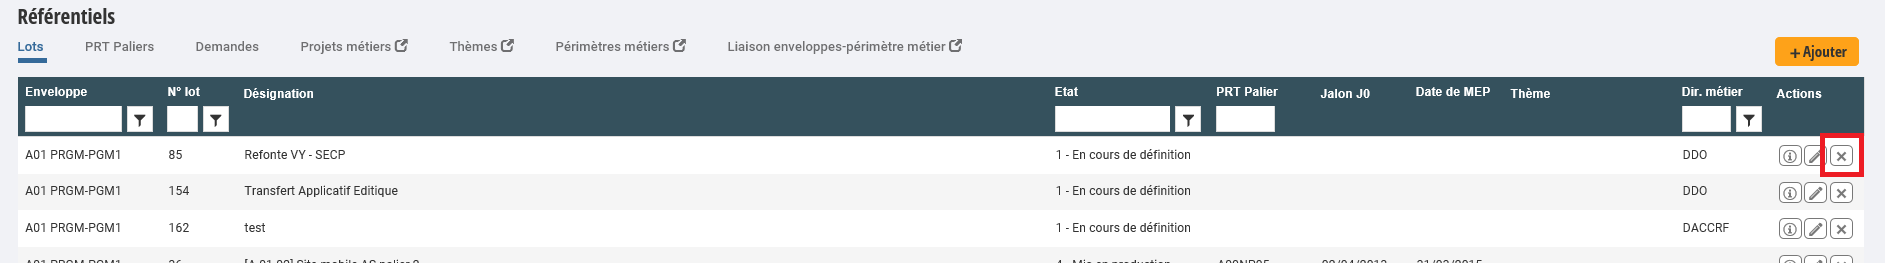
\includegraphics[width=1\textwidth]{images/ano2.png}
\caption{HPALM : Defect 2112}
\end{figure}


\subsubsection{Troisième anomalie }

\textbf{Description de l'anomalie :} En restitution d'un projet, onglet synthèse, quand on remonte sur une semaine précédente, les dates ne sont pas les bonnes. 

\begin{figure}[!h]
\centering
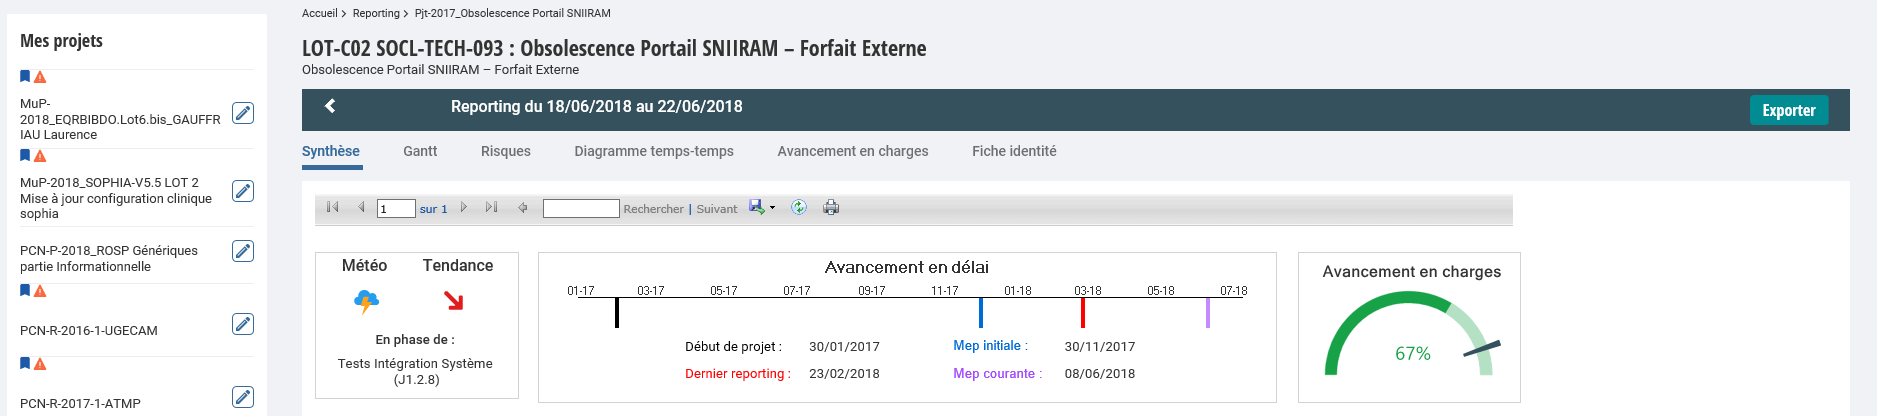
\includegraphics[width=1\textwidth]{images/ppil-indicateur-synthese.PNG}
\caption{Indicateur Synthèse}
\end{figure}

Les difficultés rencontrées lors de cette correction ont été :
\begin{itemize}
    \item Comprendre le fonctionnel, c'est à dire la logique des jalons.
    \item Travailler et modifier des requêtes complexes.
    \item Ne pas faire de régression.
\end{itemize}


\subsubsection{Des anomalies très complexes ** photo ?}

des requêtes très complexes qui vont chercher des données sur le CUBE, aucun membre de l'équipe ne maîtrise la techno, je suis chargé pendant une semaine d'analyser les ano et de trouver une correction. Un des développeur m'a rejoint pour chercher des solutions avec moi.


%%% Local Variables: 
%%% mode: latex
%%% TeX-master: "isae-report-template"
%%% End: 
\chapter{Missions complémentaires}
\label{chap:troisiemechapitre}

\section{Le projet MATRIX}

\subsection{Contexte du projet}

En plus de ma mission principale (participer aux développement de PPIL), j'ai travaillé sur le projet MATRIX. Nous avons formé une équipe de 6 stagiaires et nous nous sommes réparti différents rôles : CP(1), RF(1), RT(1), BA(2), SB(2). Mon rôle pour ce projet est celui de SB (développeur). Nous avons tous travaillé ensemble sur les différentes phases du projet. Et surtout (pour le moment) sur les phases de relation client, cadrage et conception. Dès que nous aurons fini les phases de cadrage et conception, nous allons commencer à développer. Le temps alloué pour ce projet est d'une demi-journée minimum par semaine.
 
\subsection{Étude des besoins (phase de cadrage)}

Nous avons eu une démarche de compréhension du client. Les managers de projet ont besoin de chercher des collaborateurs en fonction des compétences de ceux-ci pour créer leurs équipes.

\subsubsection{L'importance d'étudier les outils existants}

Pour réaliser cette tâche de recherche de collaborateurs répondant à certaines compétences, les managers de projets ont des outils / processus déjà existant, tels que :

Le premier outil utilisé au niveau du pôle CNAM métier étant un fichier Excel qui répertorie les compétences des collaborateurs. Cette solution pose des difficultés principalement au niveau de la maintenabilité des informations à jour.

La deuxième solution qui s'offre aux managers de projet est, dans l'intranet du groupe (tout Sopra Steria), une section de recherche d'expert en fonction d'une compétence. Cet outil ne répertorie qu'une partie des collaborateurs (les experts dans un domaine), et la localisation de ceux-ci n'est pas à jour.

\begin{figure}[!h]
\centering
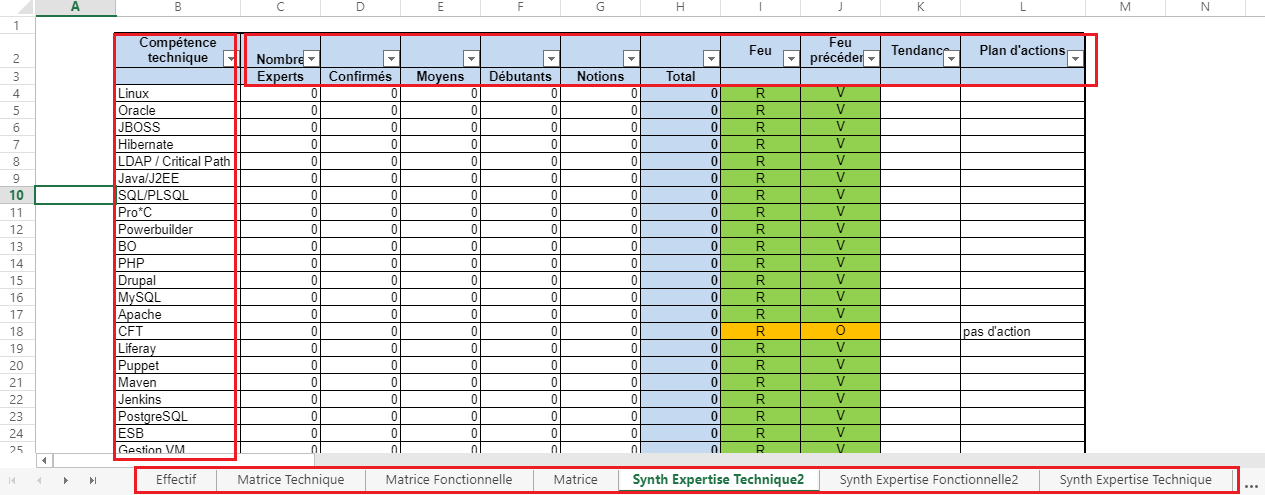
\includegraphics[width=1\textwidth]{images/MATRIX-excel.png}
\caption{MATRIX : Template du document Excel qui recense les collaborateurs en fonction de leurs compétences}
\end{figure}

Il est important d'analyser ce document car c'est celui-ci, qui dans la pratique est utilisé par les managers de projets. Pour la conception de notre application, il est important de prendre en compte la façon dont les informations sont agencées dans ce fichier Excel.

Aux vues des outils et processus cités ci-dessus, on voit bien que l'application MATRIX a sa place au sein du pôle CNAM métier et qu'elle serait un réel atout pour les managers de projets.

\subsection{Concevoir une application, notre démarche}

Lors de la conception de l'application, nous nous sommes retrouvés face à diverses problématiques. 

Par exemple, lorsque nous nous sommes demandés comment sera géré la liste des compétences en base de données : qui et comment seront ajoutées les compétences ?

Nous nous sommes retrouvés face à plusieurs questions : Est-ce qu'un utilisateur peut ajouter lui-même une fonctionnalité ? Ou bien est-ce qu'elle sont déterminées en base de données ? Si elles sont déterminées en base de données, comment en ajouter une nouvelle ? Faut-il faire des demandes administrateur ? Est-ce que les détails de la compétence (image, version) seront transmises avec ?

Toutes ces questions, nous avons pu y répondre, grâce à :
\begin{itemize}
\item l'étude des outils existants (document Excel) ;
\item différents points avec le client ;
\item priorité et faisabilité des fonctionnalités en un temps déterminé.
\end{itemize}

Nous avons choisi de :
\begin{itemize}
\item Ne pas prendre en compte les différentes versions des technologies (grâce au document Excel) ; 
\item Ne pas passer par l'administrateur pour ajouter une technologie (grâce aux entretiens avec le client) ;
\item Créer une liste par défaut des technologies en base de données (grâce au document Excel).
\end{itemize}


\subsubsection{Classer les fonctionnalités par priorité : Lot 1 et Lot 2}

Nous avons décidé que le lot 1 concernera les fonctionnalités principales et le lot 2 les fonctionnalités secondaires. Nous avons priorisé les fonctionnalités selon les besoins du client.

\subsubsection{Choix des technologies}

Nous avons été libre de choisir les technologies : 
\begin{itemize}
\item Java Spring 
\item JHipster 
\item JavaScript
\end{itemize}

Spring est un socle pour le développement d'applications très répandu en entreprise. Il représente un réel avantage en nous fournissant de nombreuses fonctionnalités qui peuvent être utilisées de plusieurs manières : ceci laisse le choix au développeur d'utiliser la solution qui correspond le plus à ses besoins.
Spring est ainsi un des frameworks le plus répandu dans le monde Java et dispose d'une grande popularité.

JHipster fournit des outils pour générer un projet avec côté client un frontal Web adaptatif (avec Angular et Bootstrap). JHipster nous permet d'atteindre nos objectif, avec plus de productivité et de qualité.

JavaScript, est le grand incontournable des pages web interactives. JHipster étant lui-même construit en parti en Angular (framework JavaScript).

\subsubsection{Mise en place des STD}

\subsubsection{Les maquettes}

Nous avons réalisé des maquettes du projet MATRIX en nous basant sur celles déjà existantes en les adaptant aux besoins du client. Ci-dessous voici deux des 7 maquettes.

\begin{figure}[!h]
\centering
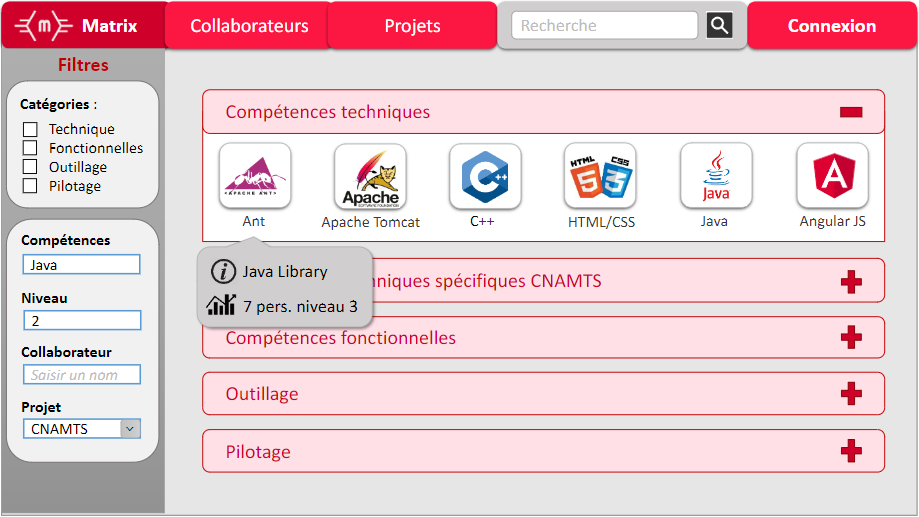
\includegraphics[width=1\textwidth]{images/matrix-maquette.png}
\caption{MATRIX : Maquette de recherche par compétence}
\end{figure}

\begin{figure}[!h]
\centering
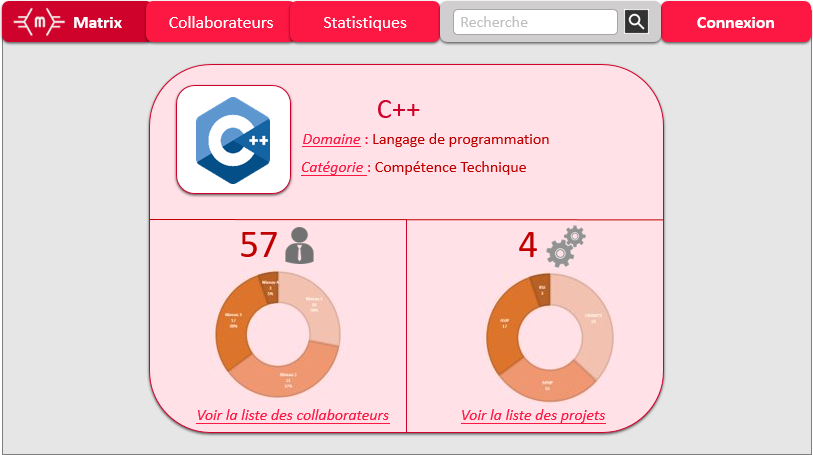
\includegraphics[width=1\textwidth]{images/matrix-maquette-competence.png}
\caption{MATRIX : Maquette détail d'une compétence}
\end{figure}

\subsubsection{La base de données}

Voici la base de données du projet :
\begin{figure}[H]
\centering
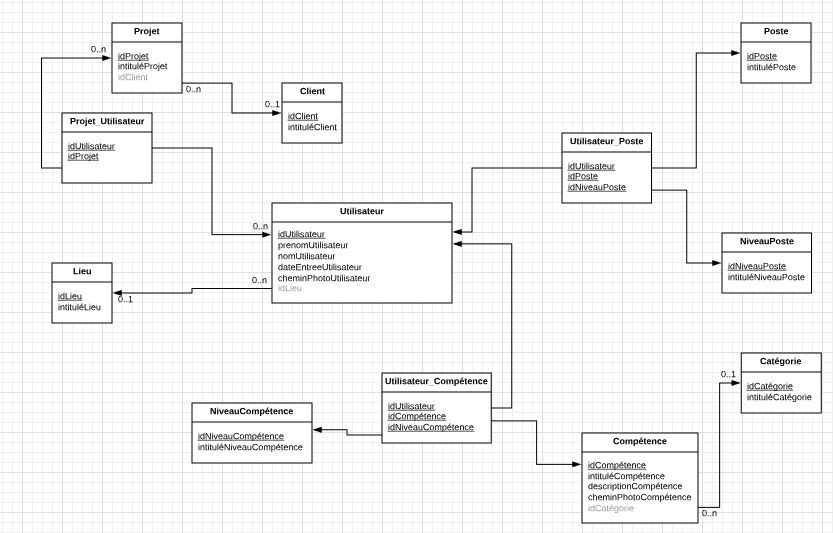
\includegraphics[width=0.8\textwidth]{images/matrix-bdd.png}
\caption{MATRIX : MCD}
\end{figure}

\subsection{Phase de développement}

\subsubsection{Installation de l’environnement}
Nous avons choisi d'utiliser l'IDE Intellij et GitLab afin de gérer nos dépots Git. Nous avons réalisé des tutoriels d'installation de nos environnements.

Nous commencerons nos développements dès que la phase de conception se terminera.

\subsection{Mise en place des SFG, STD}

Nous avons rédigé les spécifications fonctionnelles et les spécifications techniques en prenant en compte les différents lots. 

\section{Interview et présentation du métier de Business Analyste en vidéo}

Sopra Steria a proposé de réaliser une vidéo de présentation du métier de BA. Cette vidéo est destinée à présenter le métier aux nouveaux arrivants sur le pôle. Nous avons réalisé cette mission à trois. Nous avons pris l'initiative de réaliser des interview filmées de 3 collaborateurs. En parallèle, nous avons créé une animation sur l'outil Powtoon. Puis nous avons réalisé un montage vidéo en fusionnant les interview et l'animation Powtoon. Cette vidéo a été présentée à tous les acteurs du pôle Cnam Métier (plus de 100 personnes). La vidéo a été très appréciée. Cette mission a été l'occasion de découvrir le métier et d'échanger avec des collaborateurs expérimentés.

\begin{figure}[H]
\centering

\includegraphics[width=0.5\textwidth]{images/presBA.png}
\caption{Sopra Steria : Présentation du métier de BA}
\end{figure}
%%% Local Variables: 
%%% mode: latex
%%% TeX-master: "isae-report-template"
%%% End: 
\chapter*{Conclusion et perspectives}
\addcontentsline{toc}{chapter}{Conclusion}
\markboth{Conclusion}{Conclusion}
\label{sec:conclusion}

Ce rapport présente une partie du travail que j'ai réalisé au sein de Sopra Steria pendant ces deux mois de stage. J'ai beaucoup appris sur le fonctionnel du projet PPIL et les technologies utilisées pour le développement de celui-ci. J'avais pour objectif d'intégrer l'équipe PPIL et de participer à la qualification et au développement du projet. Le client est satisfait de la dernière version de PPIL qui lui a été livrée. PPIL va continuer d'évoluer avec de nouvelles fonctionnalités. A notre époque tout passe par notre smart-phone, on peut donc penser qu'une évolution mobile de restitution ou reporting des informations du portail serait la bienvenue sur mobile. J'ai également participé au cadrage et à la conception du projet MATRIX. J'entamerai les développements du projet MATRIX à partir de début juillet. 
Pour la suite de mon stage, je vais rejoindre l'équipe qui travaille sur l'application "activ'dos" afin de développer des évolutions de cette application. Une application avec plus de 100 000 téléchargements sur Google Play. J'ai de la chance d'intégrer une équipe dynamique et motivée. Je travaille sur différentes phases d'un projet et découvrir plusieurs technologies.

%%% Local Variables: 
%%% mode: latex
%%% TeX-master: "isae-report-template"
%%% End: 



\appendix

\bibliographystyle{authoryear-fr}
\bibliography{references}

%\clearpage

%%%%%%%%%%%%%%%%
%%% Abstract %%%
%%%%%%%%%%%%%%%%

%\thispagestyle{empty}
%
%\vspace*{\fill}
%\noindent\rule[2pt]{\textwidth}{0.5pt}\\
%{\textbf{Résumé ---}}
%Lorem ipsum dolor sit amet, consectetur adipiscing elit. Sed non risus. Suspendisse lectus tortor, dignissim sit amet, adipiscing nec, ultricies sed, dolor. Cras elementum ultrices diam. Maecenas ligula massa, varius a, semper congue, euismod non, mi. Proin porttitor, orci nec nonummy molestie, enim est eleifend mi, non fermentum diam nisl sit amet erat. Duis semper. Duis arcu massa, scelerisque vitae, consequat in, pretium a, enim. Pellentesque congue. Ut in risus volutpat libero pharetra tempor. Cras vestibulum bibendum augue. Praesent egestas leo in pede. Praesent blandit odio eu enim. Pellentesque sed dui ut augue blandit sodales. Vestibulum ante ipsum primis in faucibus orci luctus et ultrices posuere cubilia Curae; Aliquam nibh. Mauris ac mauris sed pede pellentesque fermentum. Maecenas adipiscing ante non diam sodales hendrerit. Ut velit mauris, egestas sed, gravida nec, ornare ut, mi. Aenean ut orci vel massa suscipit pulvinar. Nulla sollicitudin. Fusce varius, ligula non tempus aliquam, nunc turpis ullamcorper nibh, in tempus sapien eros vitae ligula. Pellentesque rhoncus nunc et augue. Integer id felis.

%{\textbf{Mots clés :}}
%Lorem ipsum dolor sit amet, consectetur adipiscing elit. Sed non risus. Suspendisse lectus tortor.
\\
\noindent\rule[2pt]{\textwidth}{0.5pt}
\begin{center}
  ISAE\\
  10, avenue Édouard Belin\\
  BP 54032\\
  31055 Toulouse CEDEX 4
\end{center}
\vspace*{\fill}

\end{document}